\documentclass[../portafolio.tex]{subfiles}



\begin{document}

\section{Método de Runge-Kutta} 

\hfill \textbf{Fecha de la actividad:} 30 de septiembre de 2022

\medskip


%---------------------------------------------------------------------------------
\subsection{Objetivo de la clase}
La finalidad de este laboratorio fue aprender a usar el método de Runge-Kutta para resolver sistemas de ecuaciones diferenciales ordinarias, específicamente las ecuaciones de Lorenz \ref{ec-lorenz1}-\ref{ec-lorenz2}. Estas ecuaciones modelan un sistema dinámico determinista tridimensional no lineal derivado de las ecuaciones simplificadas de rollos de convección que se producen en las ecuaciones dinámicas de la atmósfera terrestre \cite{ec-de-lorenz}.

\begin{align}
    \dot{x} &= \sigma (y-x),  \label{ec-lorenz1}\\
    \dot{y} &= \rho x -y -xz, \\
    \dot{z} &= xy - \beta z . \label{ec-lorenz2}
\end{align}

En las ecuaciones de Lorenz \ref{ec-lorenz1}-\ref{ec-lorenz2} $\sigma$, $\rho$ y $\beta$ son parámetros asociados al número de Prandtl y al número de Rayleigh, a estos parámetros se les asignaron los siguientes valores: $\sigma=10$, $\rho=28$ y $\beta=8/3$.

\subsection{Desarrollo del laboratorio}

Antes de comenzar a resolver las ecuaciones diferenciales ordinarias se asignaron los valores iniciales de $x$, $y$ y $z$, estos fueron $x=0$, $y=1$ y $z=1.05$. Con estos valores ya definidos se resolvió la ecuación diferencial ordinaria con ayuda del método de Runge-Kutta, para ello se creó el código \ref{c1RK}.

\begin{listing}[h]
    \begin{minted}[
frame=lines,
framesep=2mm,
baselinestretch=1.2,
bgcolor=LightGray,
fontsize=\footnotesize,
linenos
]
{python}
def f(u,t, rho=28, beta= 8/3 , sig=10):
    x,y,z = u
    return np.array([sig*(y-x), rho*x-y-x*z, x*y - beta*z ])

tmax=80
h=0.01
t= np.arange(0,tmax,h)

u=np.empty([t.size,3])
u[0]=[0,1,1.05]

for n in range(t.size-1):
    K1= f(u[n], t[n])
    K2= f(u[n] + h*0.5*K1, t[n]+0.5*h )
    K3= f(u[n] + h*0.5*K2, t[n]+0.5*h )
    K4= f(u[n] + h*K3, t[n]+h )
    u[n+1]= u[n] + (h/6)*(K1 + 2*K2 + 2*K3 + K4)
    \end{minted}
\caption{Fragmento de código que resuelve las ecuaciones de Lorenz a través del método de Runge-Kutta.}
\label{c1RK}
\end{listing}




En la primera línea del código \ref{c1RK} se creó la función $f$ que retornó un \texttt{array} de \texttt{numpy} del sistema de las ecuaciones de Lorenz, luego en la línea 5, 6 y 7 se creó un \texttt{arange} de $30000$ números que iban del $0$ al $300$. En la línea 9 se definió a $u$ como una matriz vacía de $30000$x$3$ y en la línea 10 se definieron los valores de la primera fila de $u$. Finalmente, en la línea 12 se creó un ciclo \texttt{for} que dio los valores restantes a $u$, es decir, resolvió el sistema de ecuaciones diferenciales ordinarias a través del método de Runge-Kutta.

\vspace{2mm}
Se graficó a $x$, $y$ y $z$ con los mismo valores iniciales anteriores con respecto al tiempo dando como resultados los gráficos de la figura \ref{RK_graf_ej1}. Luego, se cambiaron solo los valores iniciales quedando $x=0.4$, $y=1.2$ y $z=1$. Ahora con estos valores iniciales se volvió a graficar con respecto al tiempo quedando así los gráficos de la figura \ref{RK_graf_ej2}



\begin{figure}[h]
    \centering
    \begin{subfigure}[b]{0.3\textwidth}
        \centering
        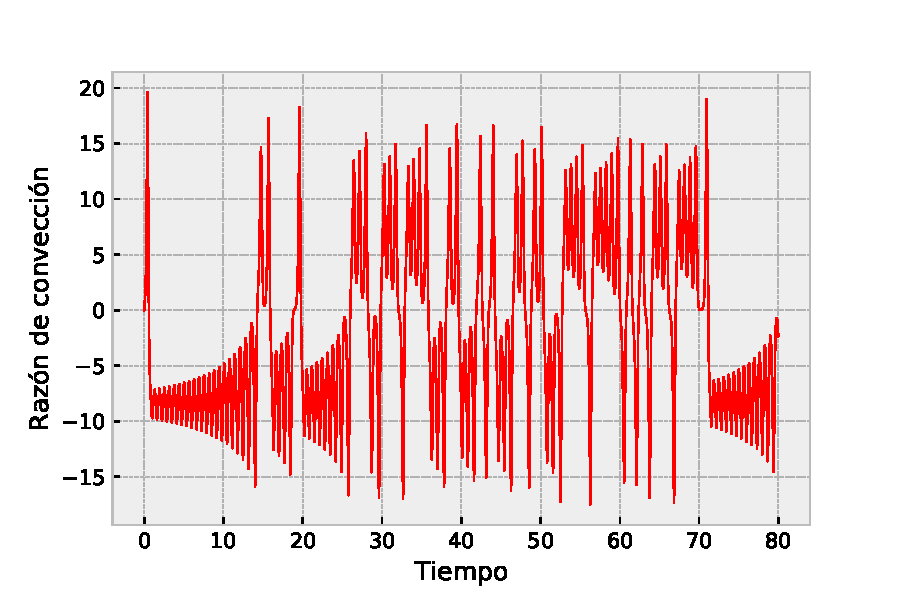
\includegraphics[width=\textwidth]{tex/img/ej2_RK_graf0.pdf}
        \caption{Gráfica de la Razón de convección con respecto al tiempo para los valores iniciales y los valores de las constantes utilizados en el código \ref{c1RK}.}
        \label{RKgraf1}
    \end{subfigure}
    \hfill
    \begin{subfigure}[b]{0.3\textwidth}
        \centering
        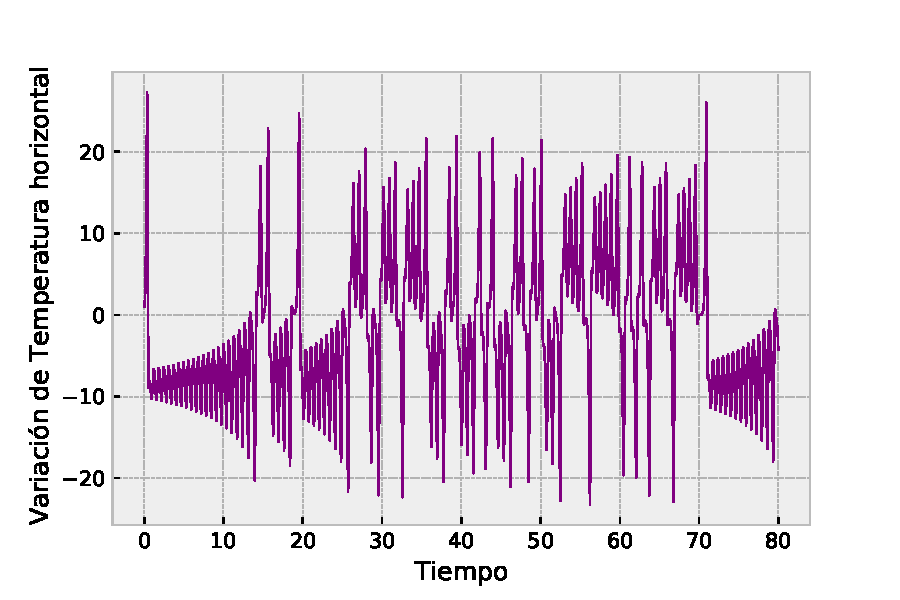
\includegraphics[width=\textwidth]{tex/img/ej2_RK_graf1.pdf}
        \caption{Gráfico de la variación de la temperatura horizontal con respecto al tiempo para los valores iniciales y los valores de las constantes utilizados en el código \ref{c1RK}.}
        \label{RKgraf2}
    \end{subfigure}
    \hfill
    \begin{subfigure}[b]{0.3\textwidth}
         \centering
         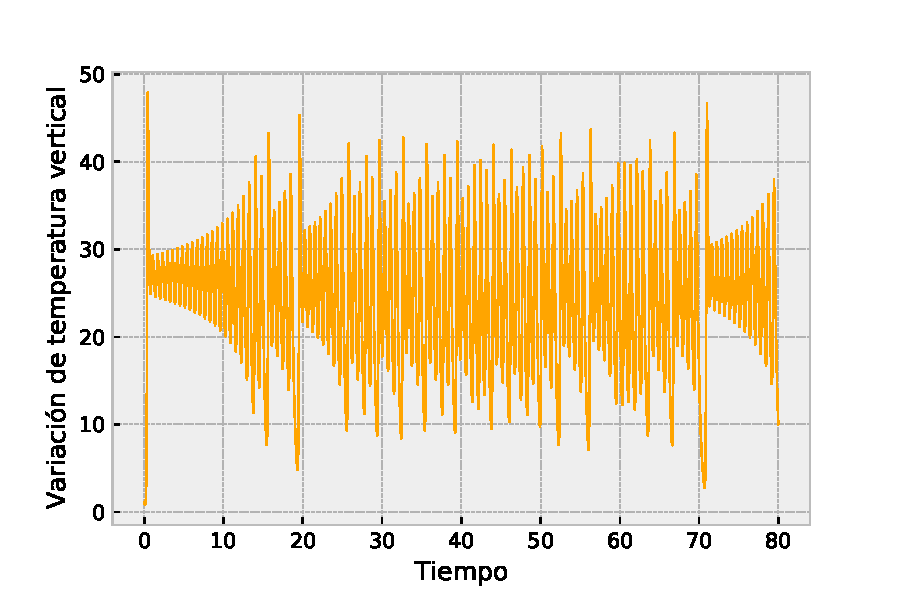
\includegraphics[width=\textwidth]{tex/img/ej2_RK_graf2.pdf}
         \caption{Gráfico de la variación de la temperatura vertical con respecto al tiempo para los valores iniciales y los valores de las constantes utilizados en el código \ref{c1RK}. }
         \label{RKgraf3}
     \end{subfigure}
    \caption{Gráficos de $x$, $y$ y $z$ con respecto al tiempo para los valores inciales $x=0$, $y=1$ y $z=1.05$.}
    \label{RK_graf_ej2}
\end{figure}

Al comparar los gráficos \ref{RKgraf1}, \ref{RKgraf2}, \ref{RKgraf3} con los gráficos \ref{RKgraf4}, \ref{RKgraf5} y \ref{RKgraf6}, respectivamente, se pudo observar claras diferencias entre ellos, de esto se pudo deducir que si las condiciones iniciales cambian, aunque sea un cambio muy pequeño, entonces se producirán cambios importantes, es decir, se está en presencia de un sistema caótico.


\begin{figure}[h]
    \centering
    \begin{subfigure}[b]{0.3\textwidth}
        \centering
        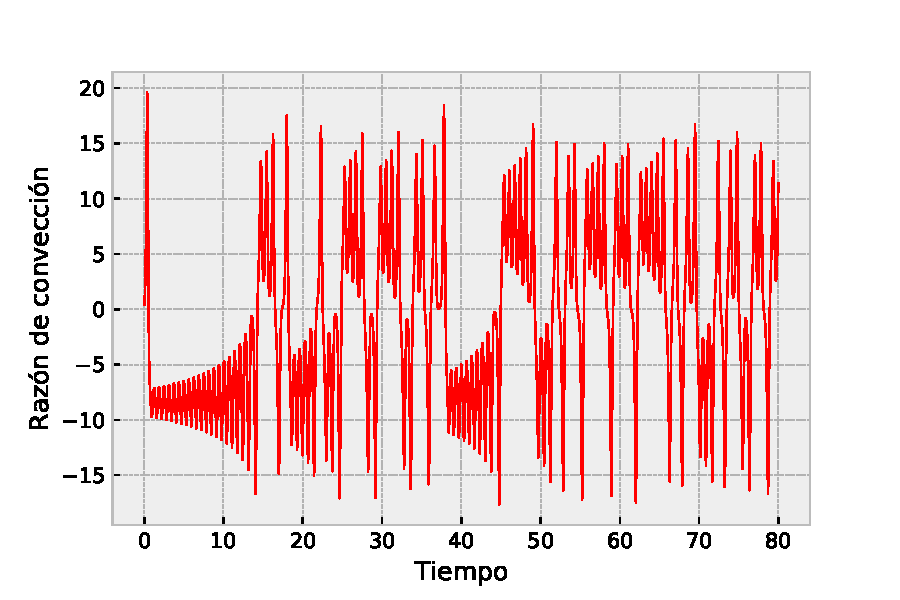
\includegraphics[width=\textwidth]{tex/img/ej2_RK_graf00.pdf}
        \caption{Gráfica de la Razón de convección con respecto al tiempo para los valores iniciales $x=1$, $y=2$, $z=1$ y los valores de las constantes utilizados en el código \ref{c1RK}.}
        \label{RKgraf4}
    \end{subfigure}
    \hfill
    \begin{subfigure}[b]{0.3\textwidth}
        \centering
        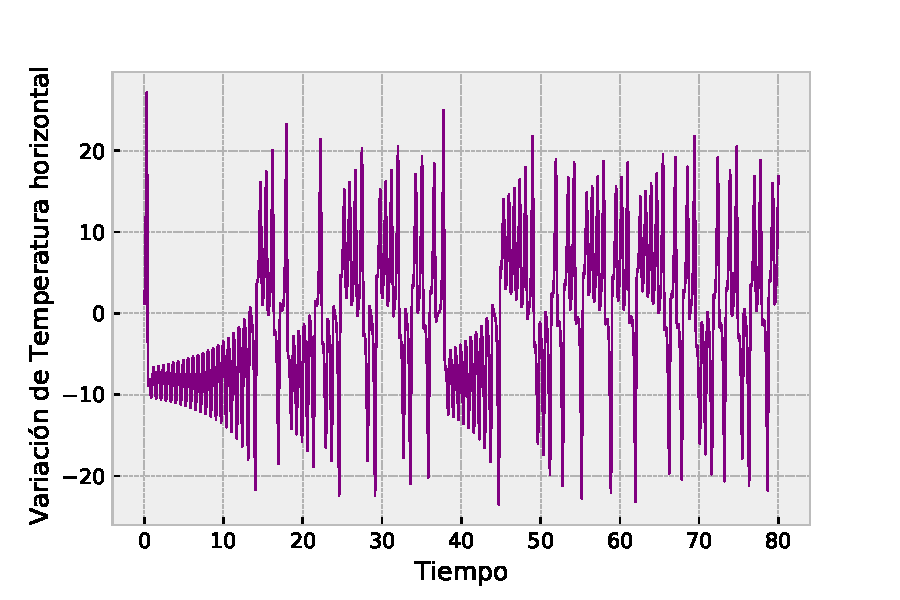
\includegraphics[width=\textwidth]{tex/img/ej2_RK_graf01.pdf}
        \caption{Gráfico de la variación de la temperatura horizontal con respecto al tiempo para los valores iniciales $x=1$, $y=2$, $z=1$ y los valores de las constantes utilizados en el código \ref{c1RK}.}
        \label{RKgraf5}
    \end{subfigure}
    \hfill
    \begin{subfigure}[b]{0.3\textwidth}
         \centering
         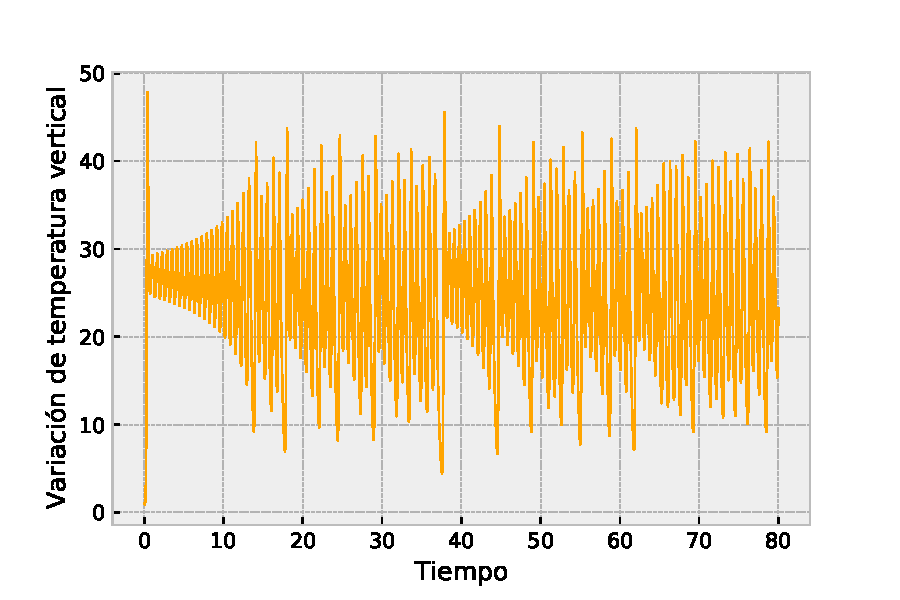
\includegraphics[width=\textwidth]{tex/img/ej2_RK_graf02.pdf}
         \caption{Gráfico de la variación de la temperatura vertical con respecto al tiempo para los valores iniciales $x=1$, $y=2$, $z=1$ y los valores de las constantes utilizados en el código \ref{c1RK}. }
         \label{RKgraf6}
     \end{subfigure}
    \caption{Gráficos de $x$, $y$ y $z$ con respecto al tiempo para los valores iniciales $x=0.4$, $y=1.2$ y $z=1$.}
    \label{RK_graf_ej1}
\end{figure}





El código \ref{c2RK} se utilizó para crear el gráfico \ref{mariposa}. En este fragmento de código se tuvieron que utilizar el paquete \texttt{matplotlib.pyplot} y la función \texttt{axes3d} del paquete \texttt{mpl\_toolkits.mplot3d}, para ello se importaron en la línea 1 y 2 del código \ref{c2RK}. En la línea 8 se definió un \texttt{array} de numpy para los valores que se graficarían en el eje $x$, lo mismos para el eje $y$ y $z$ en las líneas 9 y 10, respectivamente. Finalmente, en la línea 12 se creó el gráfico \ref{mariposa}.


\begin{listing}[H]
    \begin{minted}[
frame=lines,
framesep=2mm,
baselinestretch=1.2,
bgcolor=LightGray,
fontsize=\footnotesize,
linenos
]
{python}
import matplotlib.pyplot as plt
from mpl_toolkits.mplot3d import axes3d

fig=plt.figure()

ax1 = fig.add_subplot(111, projection="3d")

xx= np.array([u[:,0]])
yy= np.array([u[:,1]])
zz= np.array([u[:,2]])

ax1.plot_wireframe(xx, yy, zz, color="green", linewidth=0.2)
    \end{minted}
\caption{--}
\label{c2RK}
\end{listing}

\vspace{2mm}
La figura \ref{mariposa} es un gráfico tridimensional donde $x(t)$ está representado en el eje $x$, $y(t)$ en el eje $y$ y $z(t)$ en el eje z, además sus valores iniciales son los mismo que se utilizaron en la figura \ref{RK_graf_ej1}

\begin{figure}[H]
    \centering
    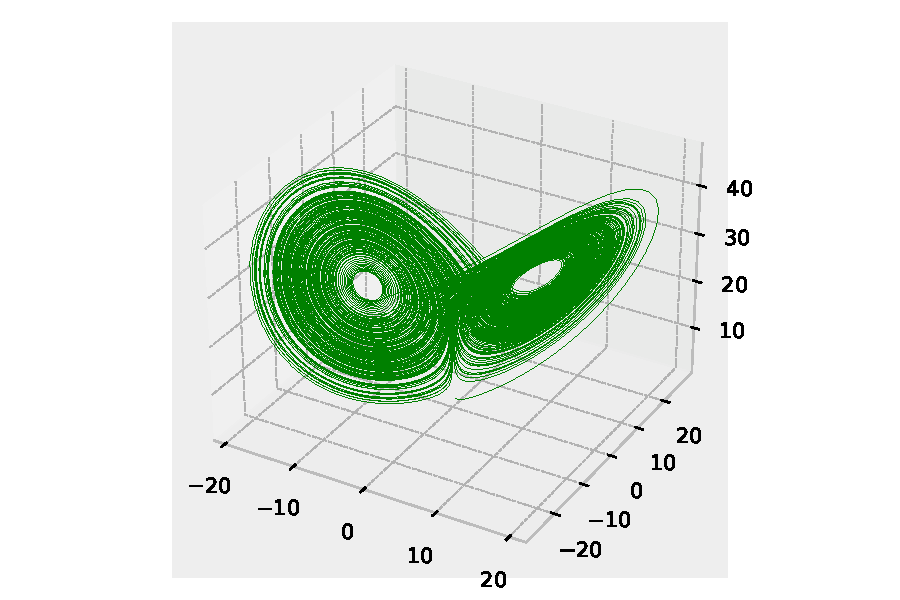
\includegraphics[scale=0.6]{tex/img/ej3_RK_graf.pdf}
    \caption{Gráfico tridimensional paramétrico de $x(t)$, $y(t)$ y $z(t)$}
    \label{mariposa}
\end{figure}




\subsection{Conclusiones}

En este laboratorio se inició resolviendo las ecuaciones de Lorenz con el método de Runge-Kutta, para ello se le asignaron ciertos valores a las constantes y a los valores iniciales, luego se graficaron las 3 ecuaciones diferenciales ordinaraias ya resueltas con respecto al tiempo. Después, se cambiaron levemente las condiciones iniciales obteniendo gráficos que diferían de los anteriores. De esto se concluyó que se estaba en presencia de un sistema complejo. Finalmente, se creó un gráfico tridimensional paramétrico de $x(t)$, $y(t)$ y $z(t)$ obteniendo las típicas alas de mariposa que caracterizan a las ecuaciones de Lorenz.

\vspace{2mm}
En esta actividad aprendí a utilizar el método de Runge-Kutta para resolver ecuaciones diferenciales ordinarias, pero esto no implica que haya entendido bien la demostración de este método, pues realmente no entendí casi nada de la demostración. Recomendaría poner quizás un poco más de énfasis en la demostración de este método para futuras realizaciones de esta actividad.



\end{document}